\documentclass[../main.tex, class=article, 12pt]{subfiles}
\usepackage{float}
\usepackage{amsthm}
\usepackage{amsmath}
\usepackage{amssymb}
\usepackage{hyperref}
\usepackage{caption}
\usepackage{mathtools}
\usepackage{graphicx}
\usepackage{todonotes}
\usepackage{tcolorbox}
\graphicspath{{./images}}




\begin{document}

Controllare il componente della vunzione vicino a $ x_0 \in dom(f) $ e confrontarlo con $ f(x_0) $.

\begin{definition}
        Controllare il comportamento della funzione vicino ad un punto $ x_0 $ che sia di \underline{accumulazione} per $ dom(f) $.
\end{definition}

\begin{definition}
        Sia $ A \subseteq \mathbb{R} \quad x_0 \in \mathbb{R}$ è detto punto di accumulazione di $ A $ se $ \forall \epsilon > 0 \quad \exists x \in A - \{x_0\} $ tale che:
        \begin{equation*}
                x_0 \epsilon \le x \le x_0 + \epsilon
        \end{equation*}
\end{definition}

\begin{exmp}
        $ A = (0, 1), x_0 = 5$ è un punto di accumulazione per $ A $.\par
\todo{25/3/22: Aggiungere retta esempio}.\newline
In questo caso per $ \epsilon < 1$ non trovo elementi di $ A $ che siano dentro $(5-\epsilon, 5+\epsilon)$. 
\end{exmp}

\begin{exmp}
        \todo{Aggiungere esempi accumulazione}
\end{exmp}

\begin{itemize}
        \item Se $ A = \mathbb{N} $ i punti di accumulazione saranno: 
                \begin{figure}[h]
                  	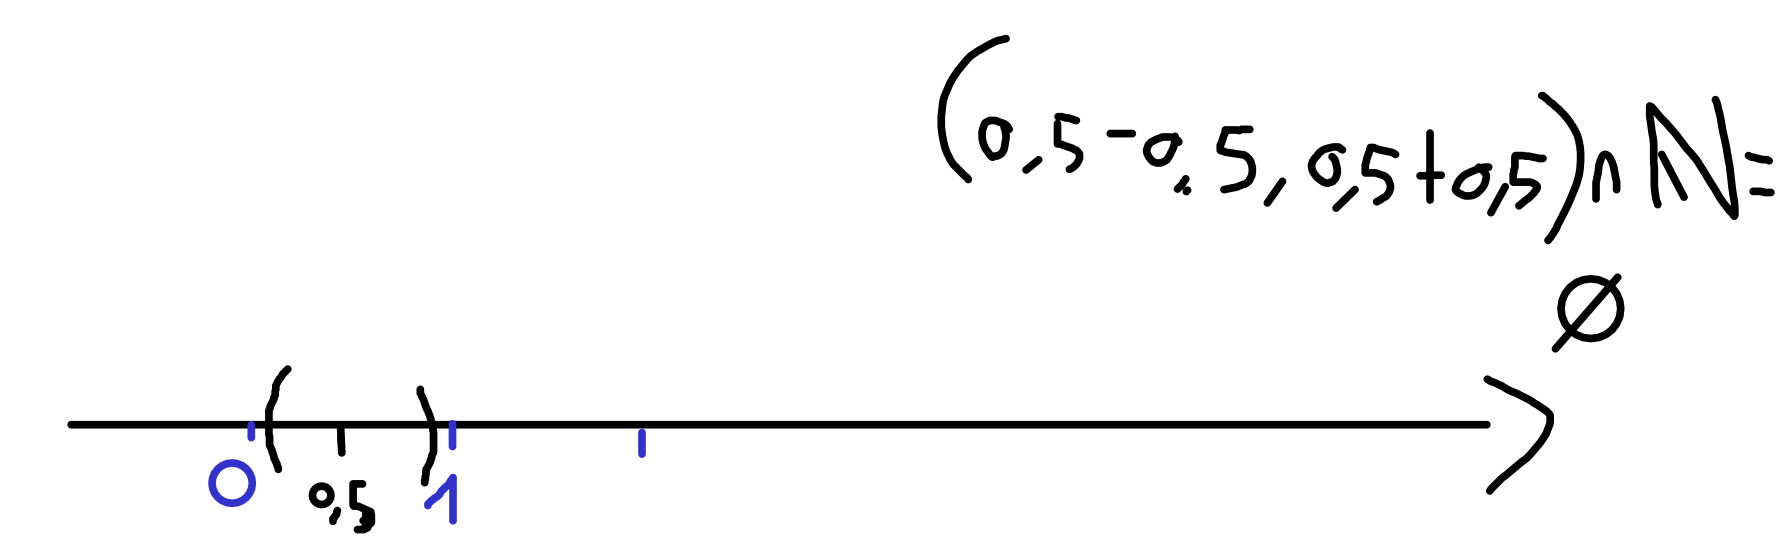
\includegraphics[width=\linewidth]{accumulazione_naturali.png}
                  	\caption{Esempio}
                        \label{fig:accumulazione_naturali}
                \end{figure}
        \item Se $ x \not \in \mathbb{N} $  allora non è di accumulazione.

        \item Se $ x \in \mathbb{N} $ non è di accumulazione se:\par $ \epsilon < 1 $ e $ g \in \mathbb{N} \quad x - \epsilon \le g \le \epsilon + x \Rightarrow g = x$ che non va bene per la definizione. 

\end{itemize}

\begin{tcolorbox}
       \textbf{NOTA:}
\end{tcolorbox}
\todo{Aggiungere nota}  


\begin{definition}
        un'altra definizione:
        \begin{itemize}
                \item $ A \subseteq \mathbb{R} $ si dice che $ a + \infty $ è punto di accumulazione di $ A $ se $ \forall M > 0 \quad  \exists x \in A$ tale che $ x \ge M $.
                \item $ - \infty $ è punto di accumulazione di $ A $ se $ \forall M>0 \quad \exists x \in A $ tale che $ x \le -M $.
        \end{itemize}
\end{definition}

Sia $ f : A \to \mathbb{R} $ e sia $ x_0 $ un punto di accumulazione di $ A $.



\subsection{Definizione di un limite}\label{sec:definizione_di_un_limite}
Avendo un limite nella forma:
\begin{equation*}
        \lim_{x \to x_0} f(x)
\end{equation*}

Possiamo ottenere quattro diverse definizioni:
\begin{enumerate}
        \item $\boxed{l \in \mathbb{R}}$
        \item $\boxed{+\infty}$
        \item $\boxed{-\infty}$
        \item \textbf{non esiste} (tipo il Molise) 
\end{enumerate}
In questi casi si può considerare $ x_0 \in \mathbb{R}, x_0 = + \infty, x_0 = -\infty$.


\subsubsection{Esempi con $ x_0 = +\infty $}
\begin{exmp}
        2:
        \begin{equation*}
               \boxed{\lim_{x \to +\infty} f(x) = +\infty}
        \end{equation*}
        \begin{figure}[H]
          	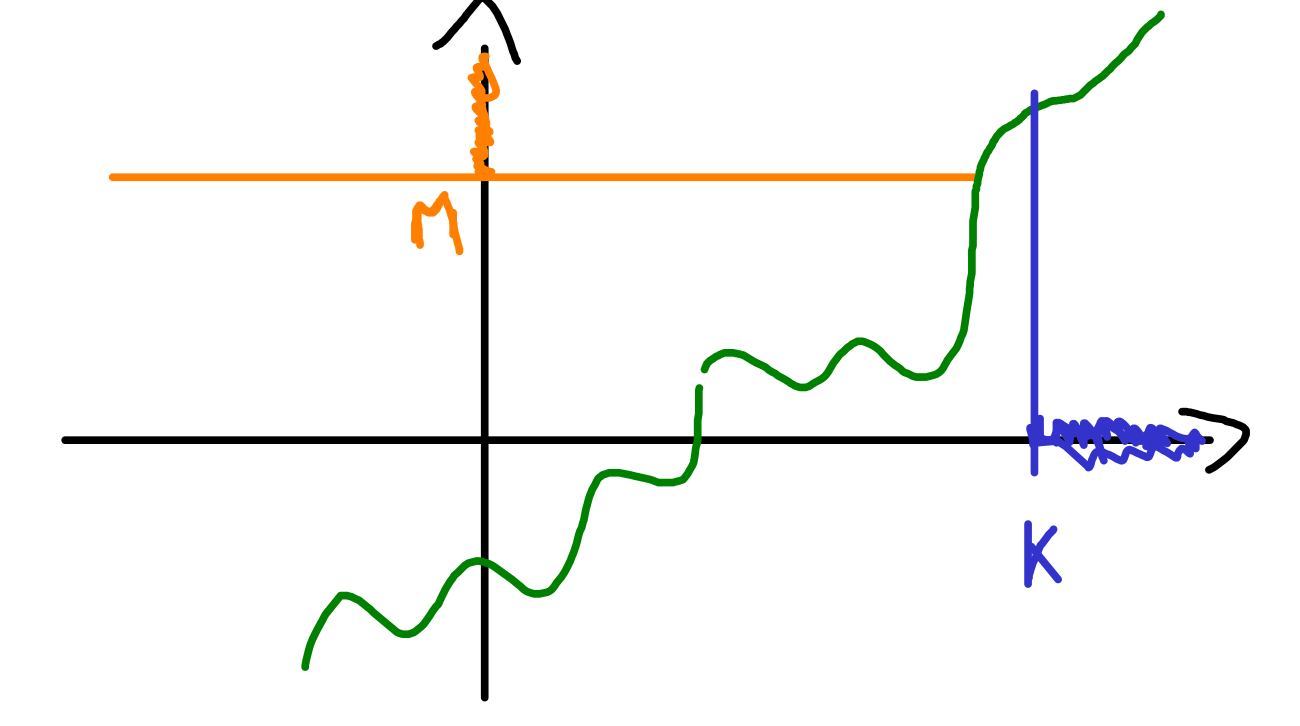
\includegraphics[width=\linewidth]{lim_es_2_+.png}
          	\caption{}
        \end{figure}
        
        $ \forall M > 0 \quad  \exists k > 0$  tale che $ \forall x \in A, x > k $ si ha:\par $ f(x) > M $. \par
        In parole semplici possiamo dire che:\par \textbf{DA UN CERTO PUNTO IN POI RESTO SEMPRE SOPRA QUALUNQUE ALTITUDINE}
\end{exmp}

\begin{exmp}
        3:
        \begin{equation*}
                \lim_{x \to +\infty} f(x) = -\infty
        \end{equation*}
        \begin{figure}[H]
          	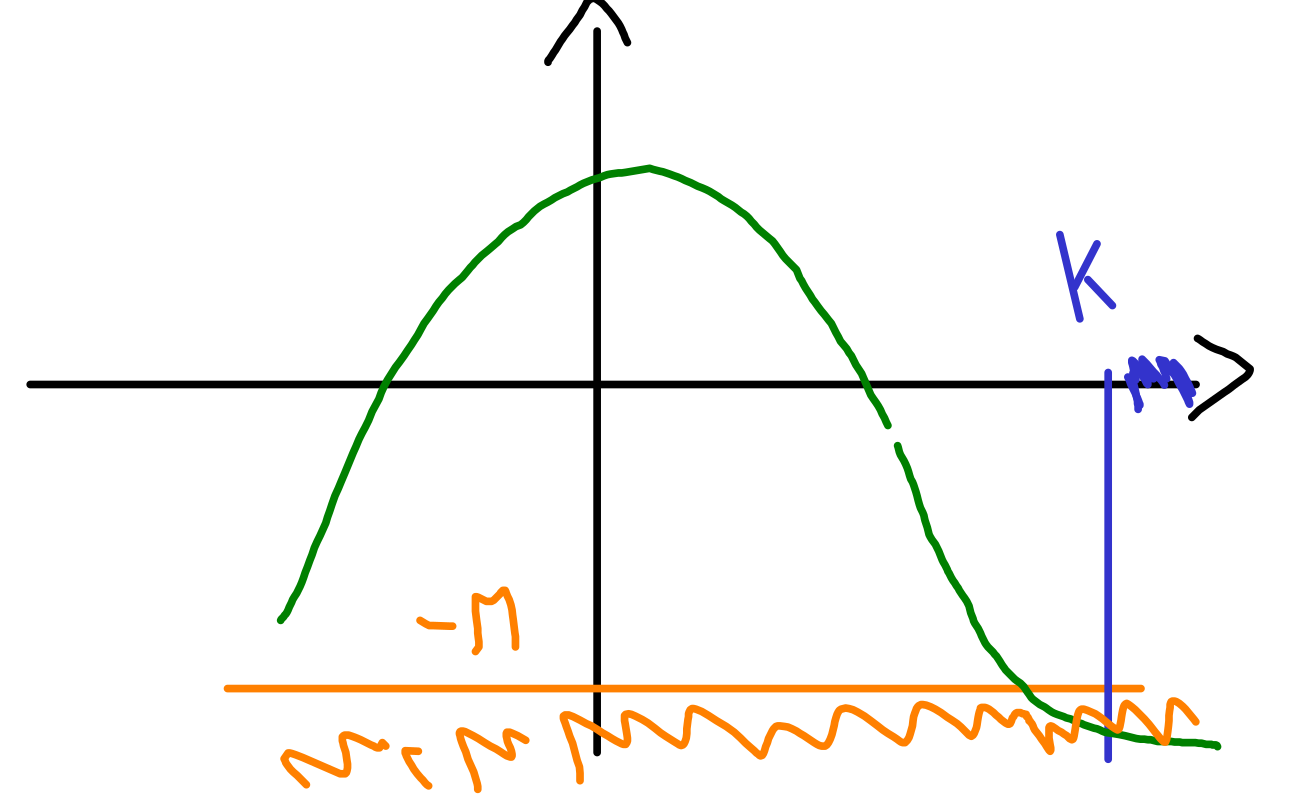
\includegraphics[width=\linewidth]{lim_es_3_+.png}
          	\caption{}
        \end{figure}
         
        $ \forall M > 0 \quad  \exists k > 0$  tale che se $ x \in A, x > k $ si ha:\par $\boxed{f(x) < -M}$. \par

\end{exmp}
\begin{exmp}
        1:
        \begin{equation*}
                \lim_{x \to +\infty} f(x) = l 
        \end{equation*}
        \begin{figure}[h]
          	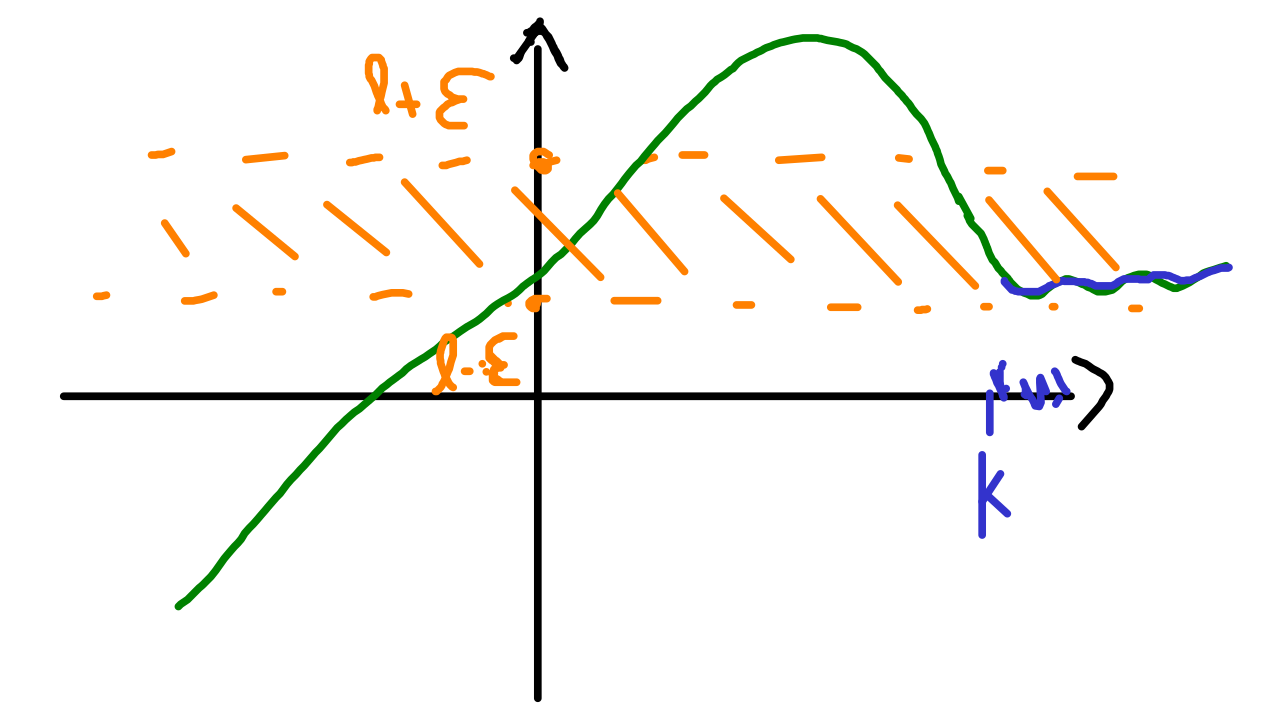
\includegraphics[width=\linewidth]{lim_es_1_+.png}
          	\caption{}
        \end{figure}
        
        $ \forall \epsilon > 0 \quad  \exists k > 0$  tale che se $\forall x \in A, x > k $ si ha:\par $\boxed{l-\epsilon<f(x) < l+\epsilon} $. \par
\end{exmp}

\begin{exmp}
        4:
        \begin{figure}[H]
          	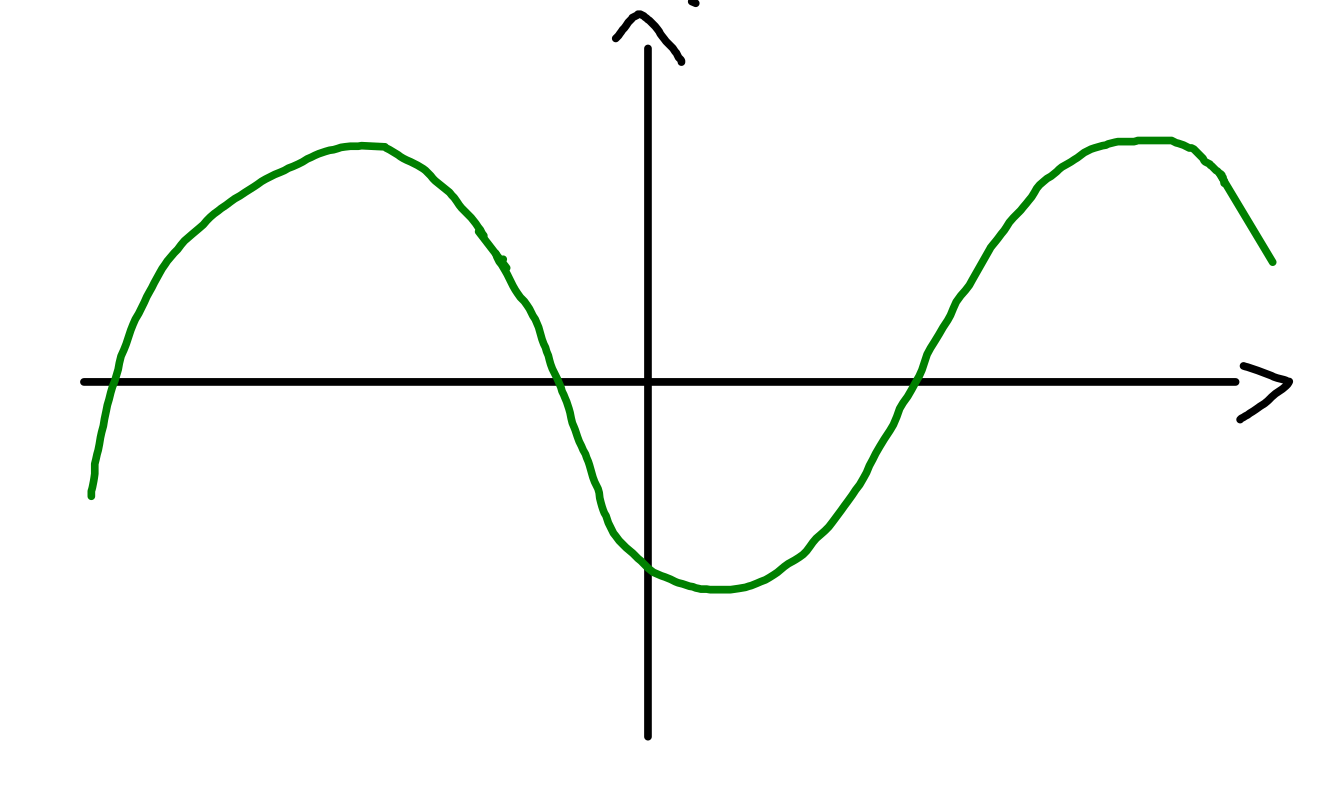
\includegraphics[width=\linewidth]{lim_es_4_+.png}
          	\caption{}
        \end{figure}
        La funzione è continua non ha limite
\end{exmp}


\subsubsection{Esempi con $ x_0 = -\infty $}
\begin{exmp}
       1:
       \begin{figure}[H]
         	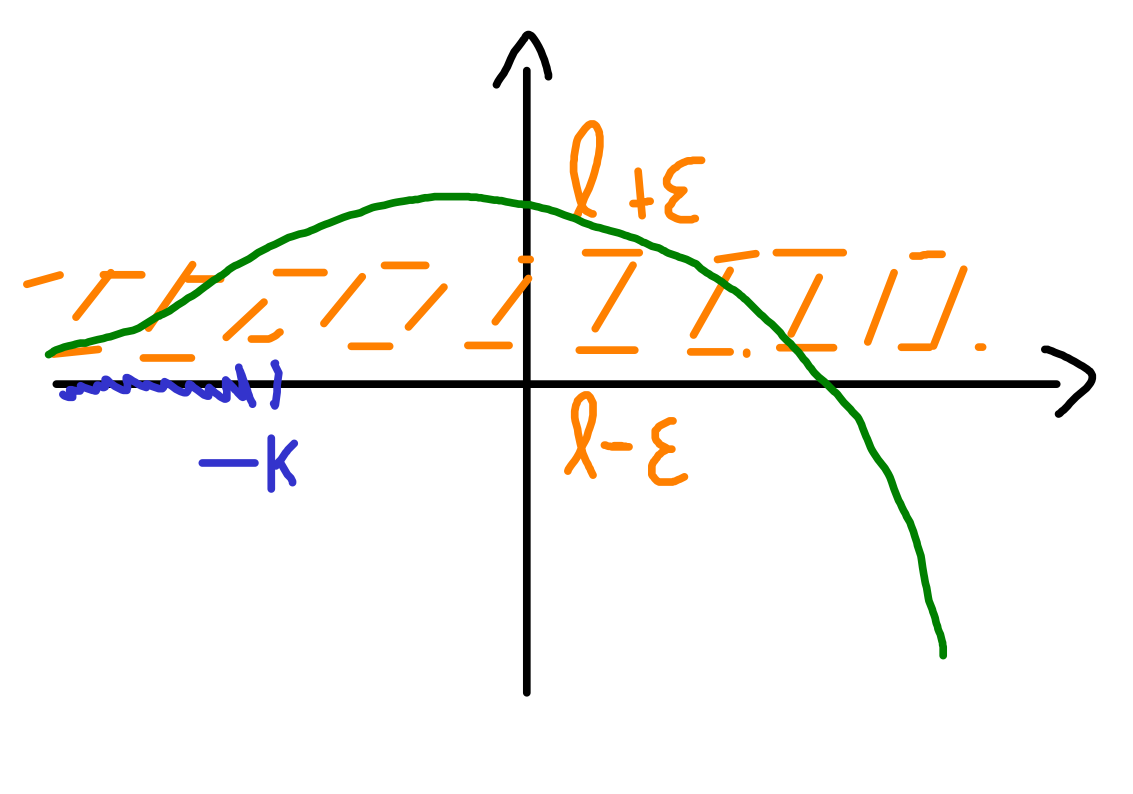
\includegraphics[width=\linewidth]{lim_es_1_-.png}
         	\caption{}
       \end{figure}
       
\end{exmp}
\begin{exmp}
       2:
       \begin{figure}[H]
         	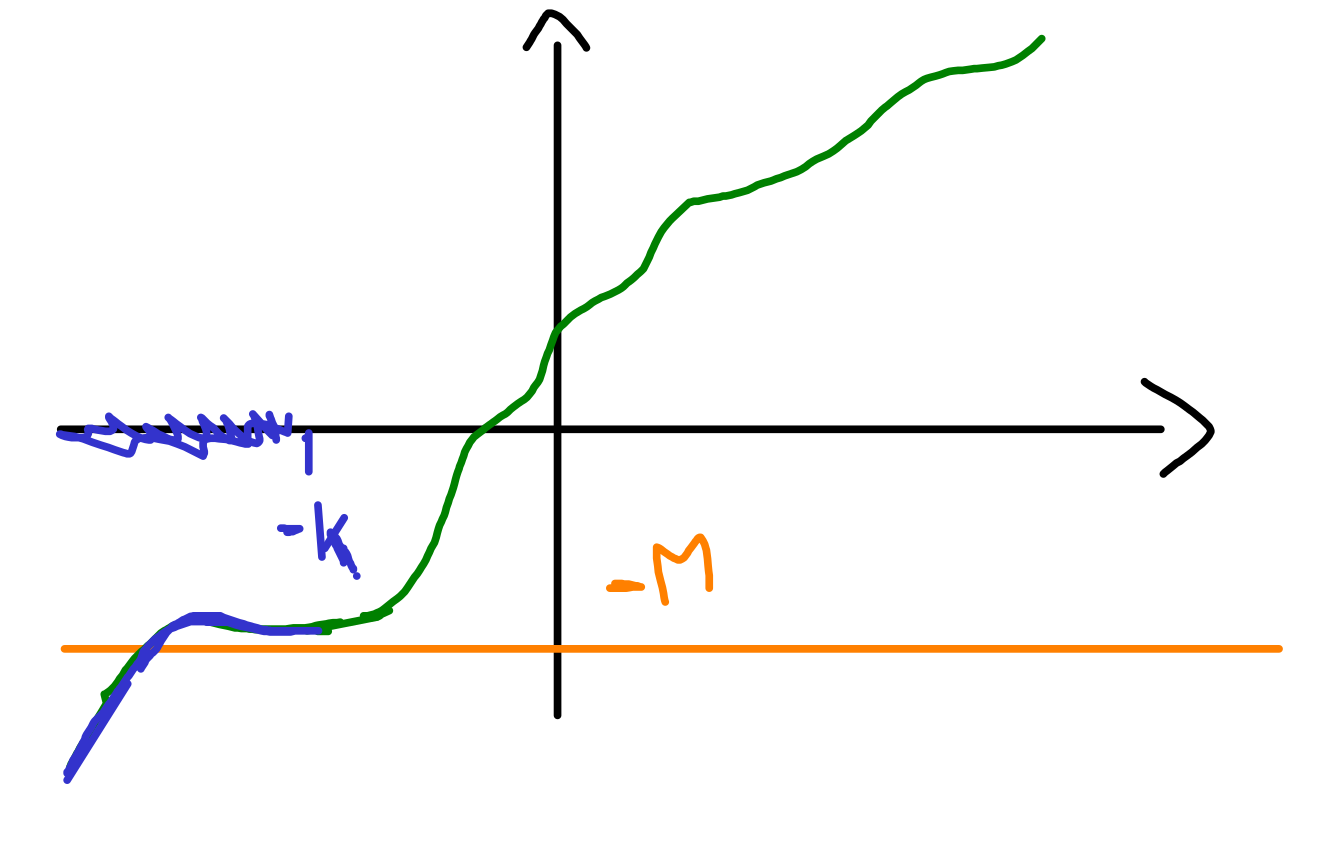
\includegraphics[width=\linewidth]{lim_es_2_-.png}
         	\caption{}
       \end{figure}
       
\end{exmp}
\begin{exmp}
       3:
       \begin{figure}[H]
         	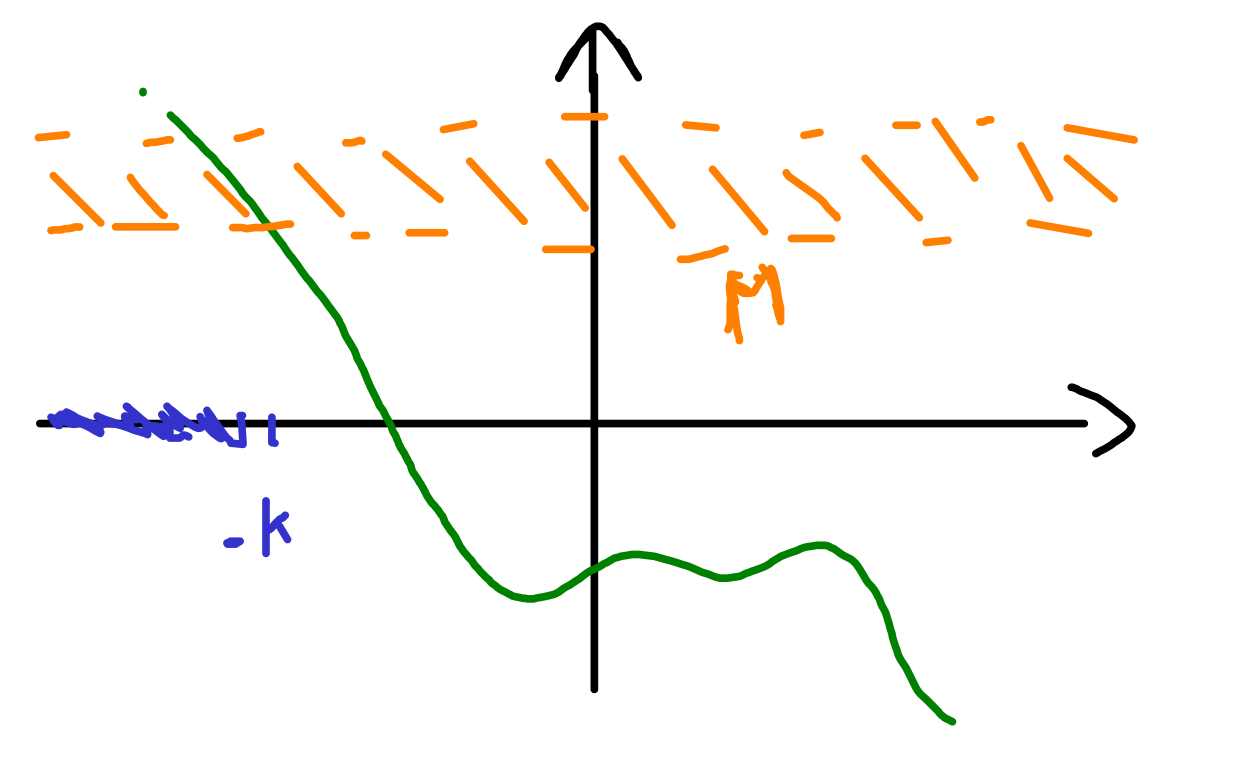
\includegraphics[width=\linewidth]{lim_es_3_-.png}
         	\caption{}
       \end{figure}
\end{exmp}
%\begin{exmp}
%       4:
%       \begin{figure}[H]
%         	\includegraphics[width=\linewidth]{lim_es_4_-.png}
%         	\caption{}
%       \end{figure}
%\end{exmp}
\todo{Aggiungere esempi  10:15}



$ \lim_{x \to 0} \not = 0 $ perchè nelle definizioni di limite non cosidero \textbf{MAI} il valore in $x = x_0$ perchè non mi interessa chi è $ f(x_0) $.

\begin{definition}
        (Continuita II) \newline
        $ x_0 \in A $ punto di accumulazione per $ A $, $ f $ è continua in $x_0$ se:
        \begin{equation*}
                \lim_{x \to x_0} f(x) = f(x_0)
        \end{equation*}
\end{definition}



\subsection{Limiti di funzioni elementari}\label{sec:limiti_di_funzioni_elementari}

Con le potenze di $ x^n \quad n \in \mathbb{N} $
\begin{align*}
        \lim_{x \to \infty} x^n > +\infty \forall n \ge 1 \\
        \lim_{x \to -\infty} x^n > +\infty \quad \forall n \ge 1 
\end{align*}



Dobbiamo prima vedere se la funzione è pari o dispari
\begin{figure}[H]
  	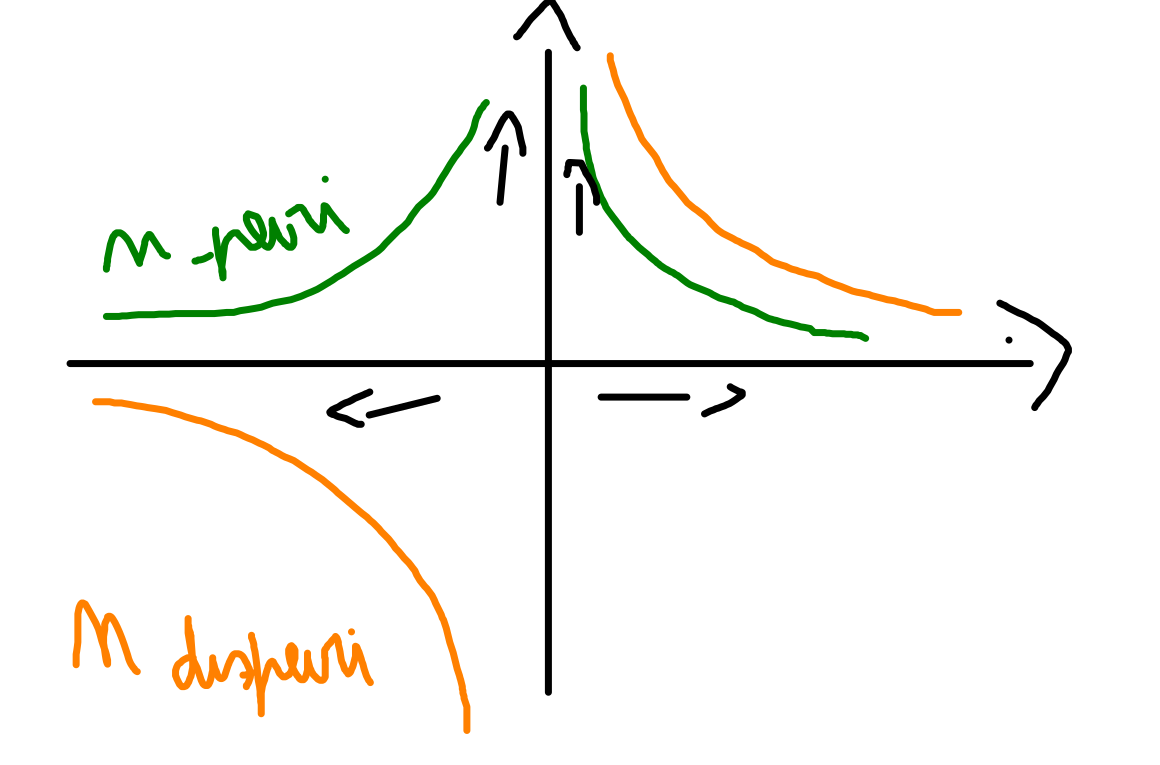
\includegraphics[width=\linewidth]{limite_pari_o_dispari.png}
  	\caption{}
\end{figure}
\todo{Recuperare i limiti}



\begin{corollario}
        $ \exists  $ intorno $ Idx_0 $, $ \exists M > 0 $ tale che:
        \begin{equation*}
                |f(x)| \le M \quad \forall I, x \not x_0
        \end{equation*}
        
\end{corollario}



\newpage
\subsection{Successioni e limiti di successioni}\label{sec:successioni}
\begin{definition}
        Una successione la possiamo immaginare come:
        \begin{align*}
                & a_1, a_2, a_3,a_4,\ldots, a_n \\
                & 1, \frac{1}{2}, \frac{1}{3}, \frac{1}{4},\ldots
        \end{align*}
\end{definition}

\begin{figure}[H]
  	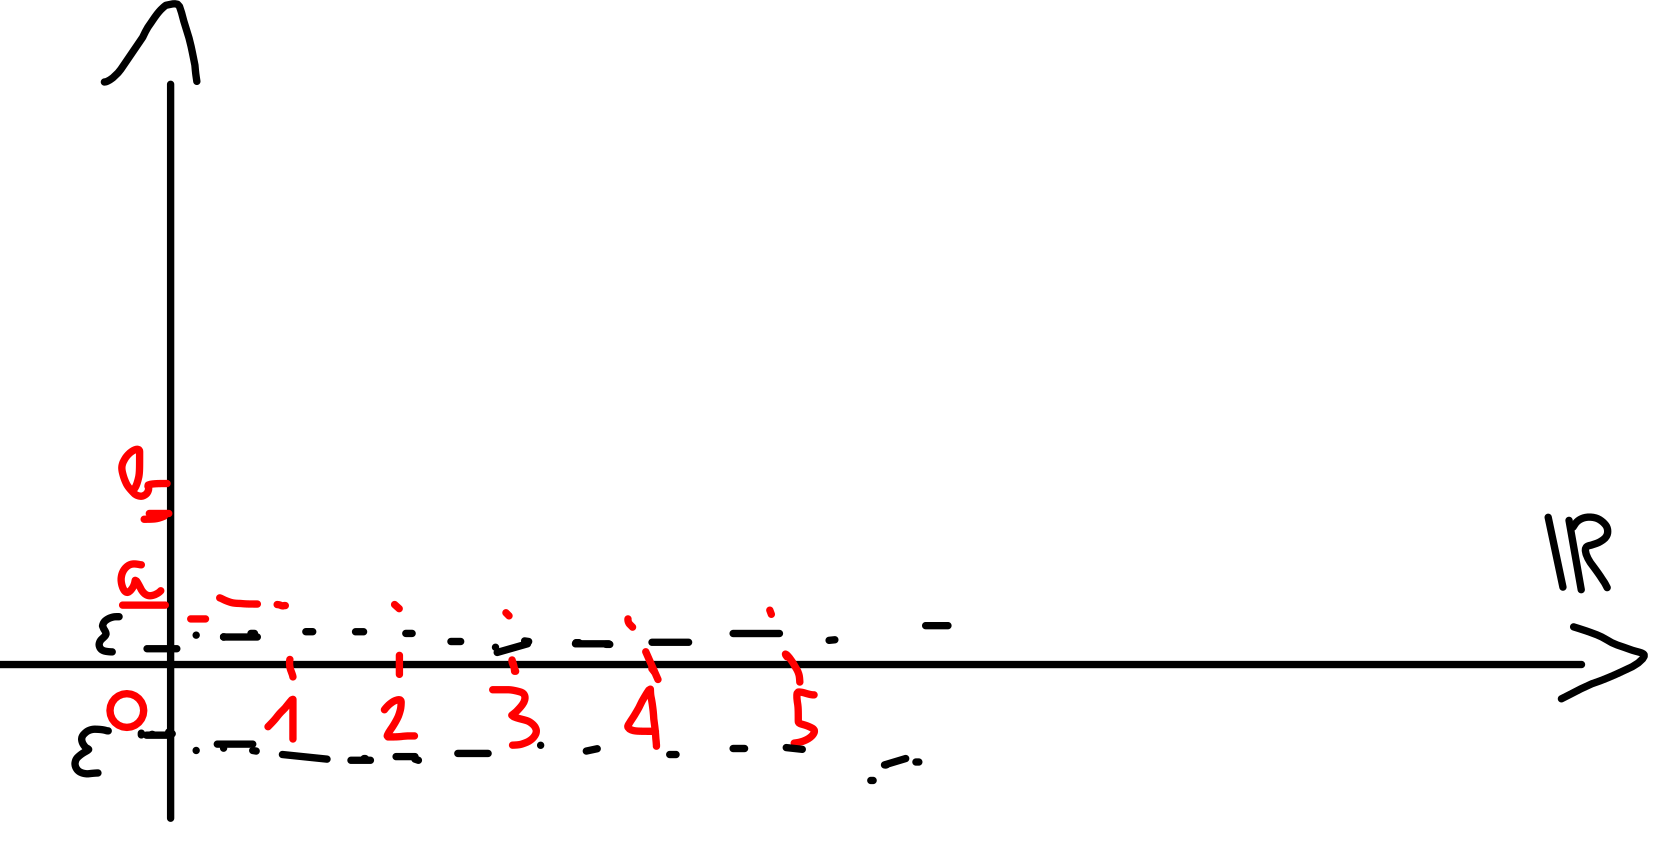
\includegraphics[width=\linewidth]{es_successioni.png}
  	\caption{}
        \label{fig:es_successioni.png}
\end{figure}

\begin{equation*}
        f : \mathbb{N} \to \mathbb{R} \quad  f(n) = a_n \quad  dom(f) = \mathbb{N}
\end{equation*}
con $ +\infty $ che è punto di accumulazione per $ A = \mathbb{N} $.

\begin{equation*}
        \lim_{n \to +\infty} a_n = l
\end{equation*}
\begin{enumerate}
        \item a
        \item b
        \item c
\end{enumerate}
\todo{LEZ 7/4: Aggiungere esempio successioni 10:30}

Valgono le stesse proprietà di limiti di funzioni, vale il teorema del confronto, teorema di permanenza del segno.





\end{document}
